\documentclass[a4paper]{article}

%% Language and font encodings
\usepackage[english]{babel}
\usepackage[utf8x]{inputenc}
\usepackage[T1]{fontenc}


%% Sets page size and margins
\usepackage[a4paper,top=3cm,bottom=2cm,left=3cm,right=3cm,marginparwidth=1.75cm]{geometry}

%% Useful packages
\usepackage{amsmath}
\usepackage{graphicx}
\usepackage{tikz,pgfplots}
\usepackage[colorinlistoftodos]{todonotes}
\usepackage[colorlinks=true, allcolors=blue]{hyperref}
\usepackage{amsfonts}
\usepackage{bbm}
\usepackage{dsfont}
\usepackage{cancel}
\usepackage{tikz,tkz-base,tkz-fct}
\newcommand{\prob}{\mathbb{P}}
\newtheorem{definicion}{Definición}
\newtheorem{teorema}{Teorema}
\newtheorem{ejemplo}{Ejemplo}
\DeclareMathOperator*{\argmax}{Arg\,max}
\newtheorem{lem}{Lemma}
\newtheorem{prop}{Proposici\'on}
\newtheorem{cor}{Corolario}
\newtheorem{dem}{Demostración}
\numberwithin{equation}{subsection}
\newtheorem{obs}{Observación}


%% Aquí se pueden definir nuevas abreviaturas para algunos comandos

\def\sen{{\rm sen\mspace{1.5mu}}}
\def\C{\mathbb C}
\def\R{\mathbb R}
\def\N{\mathbb N}
\def\Q{\mathbb Q}
\def\Z{\mathbb Z}
\def\V{\mathbb V}
\def\E{\mathbb E}
\def\to{\rightarrow}
\newcommand{\pb}{\mathbb{P}}



\newcommand{\ds}{\displaystyle}


%Para hacer normas en tex

\providecommand{\norm}[1]{\lVert#1\rVert}
\providecommand{\normm}[1]{\bigg\lVert#1\bigg\rVert}


%integrales bacanes
\usepackage{ esint }

%Para poner en negrita en modo matemático
\newcommand{\negri}{\boldsymbol}




\title{Simulación Estocástica}
\author{Clase 2}
\date{1 de agosto de 2019}

\begin{document}
\maketitle

\section{Notación}
\begin{itemize}
    \item $c.s.$: "Casi seguramente"
\end{itemize}

\textbf{Demostración (Portmanteau):} Dado que las funciones uniformemente contínuas, en particular son contínuas, la implicancia $i)\rightarrow ii)$ se desprende trivialmente de la definicion de convergencia débil en $i)$. Así mismo la implicancia $ii) \rightarrow iii)$ considerando las funciones Lipschitz.\\
Veamos la implicancia $iii) \rightarrow iv)$: \\ \newline
Sea $F$ un conjunto cerrado. $\forall \epsilon > 0$, sea:
\begin{equation}
   f(x) = \max\left(1-\frac{d(x,F)}{\epsilon}, 0\right)
   \label{eq:dem1}
\end{equation}

Donde $d(x,F)$ está dado por la métrica del espacio $E$. Se puede probar que la función $f$ definida de esta forma es $\frac{1}{\epsilon}$-Lipschitz y vale 1 en todo $F$. Además:
\begin{equation}
    \mathbbm{1}_F \leq f \leq \mathbbm{1}_{F^{\epsilon}}\hspace{1cm}\text{donde }F^{\epsilon}:=\{x\in E\,|\,d(x,F)<\epsilon\}\
    \label{eq:demostracionprtmanteau}
\end{equation}
Luego, integrando (bajo $\mu_n$) en las dos primeras partes de la desigualdad y aplicando límite superior:
\[\limsup\,\mu_n(F)\leq \limsup\,\langle \mu_n,f\rangle\]
Pero, como habíamos dicho, al ser $f$ una función Lipschitz, por la proposición $iii)$; $\langle \mu_n,f\rangle$ converge, por lo tanto el límite superior en realidad es el límite, más aún, converge en términos de $\mu$:
\begin{equation}
    \limsup \langle \mu_n,f\rangle = \lim \langle\mu_n,f\rangle = \langle \mu,f\rangle
\end{equation}
Ahora, nuevamente por la expresión en \ref{eq:demostracionprtmanteau}, integrando la segunda desigualdad (ahora bajo $\mu$):
\[\langle\mu,f\rangle \leq \mu(F^{\epsilon})\]
En resumen, tenemos que:
\[\limsup\,\mu_n(F) \leq \langle\mu,f\rangle \leq\mu(F^{\epsilon})\]
Al ser $F$ cerrado y $F^{\epsilon} \searrow F$, por continuidad de la medida se tiene que $\mu(F^{\epsilon})\searrow \mu(F)$ al momento que $\epsilon \rightarrow 0$ concluyendo el resultado.

\begin{figure}
\centering
    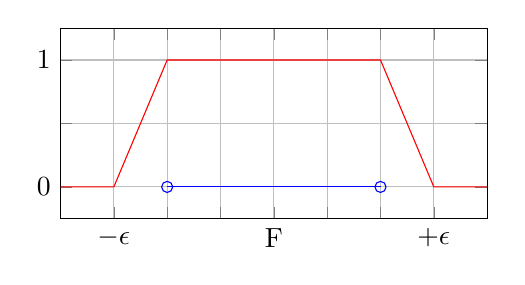
\begin{tikzpicture}
         \begin{axis}
        [width=7cm, height=4cm, xmin=-1, xmax=1, ymin=-0.25, ymax=1.25, xmajorgrids=true, ymajorgrids=true, xtick={-1,-0.75,-0.5,-0.25,0,0.25,0.5,0.75,1},  xticklabels={,$-\epsilon$,,,F,,,$+\epsilon$,}, ytick={0,0.5,1}, yticklabels={0,,1}]
        \addplot[color=red] coordinates {(-1,0) (-0.75,0) (-0.75,0) (-0.5,1) (-0.5,1) (0.5,1) (0.5,1) (0.75,0) (0.75,0) (1,0)};
        \addplot[color=blue, mark = o] coordinates {(-0.5,0) (0.5,0)};
        \end{axis}
    \end{tikzpicture}
    \caption{Esquema función f en \ref{eq:dem1}}
\end{figure}
\newpage
Es directo ver que la proposición $iv)$ y $v)$ son equivalentes, así que la implicancia $iv) \rightarrow v)$ es directa de tomar complemento y utilizar que $\mu_n$ y $\mu$ son medidas de probabilidad.\\ \newline
Veamos que $iv)\land v)$ implican a $vi)$: Sea $A$ un conjunto $\mu$-contínuo. Dado que $\Bar{A}$ es cerrado, $A^{\circ}$ es abierto, ocupando la proposición $iv)$ y $A^{\circ} \subset A\subset \Bar{A}$:
\[\mu(\Bar{A}) \geq \limsup\,\mu_n(\Bar{A}) \geq \limsup\,\mu_n(A)\geq \liminf\,\mu_n(A) \geq \liminf\,\mu_n(A^{\circ})\geq \mu(A^{\circ})\]
Además, como $A$ es $\mu$-contínuo: $\mu(\partial A) = 0$, entonces $\mu(\Bar{A}) = \mu(A^{\circ}) = \mu(A)$, por lo tanto todas las desigualdades anteriores son, en realidad, igualdades. Concluímos así que:
\begin{itemize}
    \item $\liminf\,\mu_n(A) = \limsup\,\mu_n(A)$ por lo tanto el límite existe.
    \item $\mu(A)\geq \lim\,\mu_n(A)\geq \mu(A)$, por lo tanto $\lim\,\mu_n(A) = \mu(A)$.
\end{itemize}
Por último, para finalizar, veremos la implicancia $vi)\rightarrow i)$:\\ \newline
Sea $f\in C_b(E)$, sin pérdida de generalidad podemos suponer que $0\leq f\leq 1$. En caso contrario, como $f$ es una función acotada, su supremo e ínfimo son finitos, por lo tanto podríamos definir una normalización para $f$:
\[\Tilde{f} = \frac{f - \inf_x f}{\sup_x f - \inf_x f}\]
Para la siguiente demostración haremos uso del siguiente resultado:
\begin{prop} Sea $g$ una función positiva, entonces:
    \begin{equation}
        \E_{\mu}(g(X)) = \langle\mu,g\rangle = \int_0^{\infty}\mu(g>t)dt
    \end{equation}
\end{prop}
\textbf{Demostración (proposición):} La primera igualdad es la definición de esperanza:
\[\E_{\mu}(g(X)) = \int_{0}^{\infty}g(x)\mu(dx)\]
donde $\mu(dx)$ puede ser escrito en función de la densidad de distribución asociada a la medida de probabilidad $\mu(dx) = h(x)dx$. Así la integral de la esperanza puede ser escrita de la forma:
\[\E_{\mu}(g(X)) =\int_{0}^{\infty}g(x)h(x)dx\]
Al mismo tiempo, podemos reescribir la función $g$ de la forma:
\[\E_{\mu}(g(X)) = \int_{0}^{\infty}\left(\int_{0}^{g(x)}dt\right)\,h(x)dx\]
Ahora podemos extender la integral en $dt$ a todo el intervalo positivo mediante una indicatriz que anule los valores superiores a $g(x)$, esto es:
\[\E_{\mu}(g(X)) = \int_{0}^{\infty}\left(\int_{0}^{\infty}\mathbbm{1}_{\{g>t\}}dt\right)h(x)dx = \int_{0}^{\infty}\int_{0}^{\infty}\mathbbm{1}_{\{g>t\}}h(x)dtdx\]
Ocupando el teorema de Fubini podemos intercambiar el orden de las integrales, entonces:
\[\E_{\mu}(g(X)) = \int_{0}^{\infty}\int_{0}^{\infty}\mathbbm{1}_{\{g>t\}}h(x)dtdx = \int_{0}^{\infty}\int_{0}^{\infty}\mathbbm{1}_{\{g>t\}}h(x)dxdt = \int_{0}^{\infty}\left(\int_{0}^{\infty}\mathbbm{1}_{\{g>t\}}\mu(dx)\right)dt\]
\[ = \int_{0}^{\infty}\mu(g>t)dt\]
\rule{0.7em}{0.7em}

Entonces, volviendo a la demostración del teorema, tenemos que:
\[\langle \mu,f\rangle = \int_{0}^{1}\mu(f>t)dt\]
\[\langle \mu_n , f \rangle = \int_{0}^{1}\mu_n(f>t)dt\]
Donde el intervalo de integración lo podemos acotar, puesto que definimos el rango de la función $f$ en $[0,1]$. Además, como $f$ es contínua, es fácil ver que:
\[\partial \{f>t\} \subset\,\{f=t\}\]
Notemos que $\mu(f=t)=0$ salvo para, a lo más numerables, valores de t's. De lo contrario, la medida $\mu$ no sería finita. Luego, $dt-c.s.$ tenemos:
\[\mu(\partial\{f>t\}) \leq \mu(\{f=t\}) = 0\]
Es decir: de manera $dt-c.s.$ $\{f>t\}$ es $\mu$-contínuo. Por la proposición $vi)$:
\[\mu_n(f>t) \xrightarrow{\,\,n\,\,}\,\mu(f>t)\hspace{1cm}dt-c.s.\]
Finalmente, ocupando el \textbf{T.C.D.}:
\[\langle\mu_n,f\rangle = \int_{0}^{\infty}\mu_n(f>t)dt \xrightarrow{\,\,\,\textbf{T.C.D.}\,\,\,}\int_{0}^{\infty}\mu(f>t)dt = \langle \mu,f\rangle\]
\rule{0.7em}{0.7em}

Habiendo establecido anteriormente, la equivalencia entre la convergencia débil de medidas de probabilidad y la convergencia en LEY de variables aleatorias, podemos enunciar el Teorema Portmanteau para variables aleatorias.

\begin{teorema}[Portmanteau para variables aleatorias.] Sean $(X_n)_{n\in\N}$, $X$ variables aleatorias en $(E,d)$ espacio métrico. Las siguientes proposiciones son equivalentes:
\begin{enumerate}
    \item[i)] $X_n\,\xrightarrow{\mathcal{L}}\,X$
    \item[ii)] $\E(f(X_n)) \xrightarrow{\,\,n\,\,}\E(f(X))$ para toda función $f$ acotada y uniformemente contínua.
    \item[iii)] $\E(f(X_n)) \xrightarrow{\,\,n\,\,}\E(f(X))$ para toda función $f$ Lipschitz.
    \item[iv)] $\limsup\,\pb(X_n \in F) \leq \pb(X\in F)$ $\forall F\subset E$ cerrado.
    \item[v)] $\liminf\,\pb(X_n \in G) \geq \pb(X \in G)$ $\forall G\subset E$ abierto.
    \item[vi)] $\lim \pb(X_n \in A) = \pb(X\in A)$ para todo $A\in \mathcal{B}(E)$ conjunto $\mu$-contínuo ( $\pb(X \in \partial A) = 0$ ).
\end{enumerate}
\end{teorema}

\begin{obs} Tomando $E=\R$, la condición $vi)$ del teorema suele ser interesante, como en el siguiente ejemplo:\\ Sabemos de ejemplos anteriores que:
\[\delta_{1/n}\Rightarrow \,\delta_{0}\]
Sin embargo, para el conjunto $A=(0,\infty)$, $\forall\,n\in\N$:
\[\delta_{1/n}(A) = 1\]
\[\delta_{0}(A) = 0\]
Es decir que $\delta_{1/n}(A)$ no converge a $\delta_{0}(A)$, sin embargo esto no contradice la condición $vi)$, pues el conjunto $A$ no es $\delta_0$-contínuo.
\[\delta_{0}(\partial A) = \delta_{0}(\{0\}) = 1\]
\end{obs}

\subsubsection{El Teorema del Mapeo.}
Supongamos que $h$ es una función de $(E,d)$ a otro espacio métrico, $(\hat{E},\hat{d})$. \\Si $h$ es $\mathcal{B}(E)/\mathcal{B}(\hat{E})$-medible, entonces cada medida de probabilidad $\mu \in \mathcal{P}(E)$ induce a otra medida de probabilidad $\mu h^{-1} \in \mathcal{P}(\hat{E})$, definida de la manera usual, como $\mu h^{-1}(A) = \mu(h^{-1}(A))$. \newpage Necesitamos, entonces, condiciones bajo las cuales el hecho de tener una convergencia débil, $\mu_n \Rightarrow \mu$, en $\mathcal{P}(E)$, me implique una convergencia débil, $\mu_nh^{-1} \Rightarrow \mu h^{-1}$ para medidas en $\mathcal{P}(\hat{E})$. \\ \newline
Una de las condiciones pensadas para $h$ podrías ser la continuidad, pero veremos que esta condición puede ser reemplazada por una más débil. Asumimos que $h$ será una función $\mathcal{B}(E)/\mathcal{B}(\hat{E})$-medible, y sea $D_h$ el conjunto de los puntos de discontinuidad de la función $h$ ($D_h \in \mathcal{B}(E)$). Tenemos el siguiente resultado;  si $\mu_n \Rightarrow\,\mu$ y $\mu(D_h) = 0$, entonces $\mu_n h^{-1} \Rightarrow\, \mu h^{-1}$. \\ \newline
En otras palabras:

\begin{teorema}[Del Mapeo.] Sea $(\hat{E},\hat{d})$ otro espacio métrico y sea $h:\,E\rightarrow\,\hat{E}$, una función medible. $(X_n)_{n\in\N}$, $X$ son variables aleatorias en $E$.\\ \newline
Si $X_n\,\xrightarrow{\mathcal{L}}\,X$ y $\pb(X \in D_h) = 0$, entonces: $h(X_n) \,\xrightarrow{\mathcal{L}}\,h(X)$. Donde $D_h :=\{x\in E\,|\,\text{$h$ es discontínua en x}\}$
\end{teorema}

\textbf{Demostración:} Sea $B \subset\,\hat{E}$, un conjunto $\mathcal{L}(h(X))$-contínua, es decir:
\begin{equation}
    \pb(h(X) \in \partial B) = 0
    \label{eq:dem2}
\end{equation}
Por el teorema Portmanteau en variables aleatorias, la convergencia el LEY es equivalente a decir que:
\[\pb(h(X_n)\in B) \xrightarrow{\,\,n\,\,}\,\pb(h(X)\in B)\]
Lo que a su vez, es equivalente a decir que:
\[\pb(X_n \in h^{-1}(B)) \xrightarrow{\,\,n\,\,}\,\pb(X \in h^{-1}(B))\]
Luego, basta con demostrar que $h^{-1}(B)$ es un conjunto $\mathcal{L}(X)$-contínuo, $i.e.$; falta por demostrar que $\pb(X \in \partial h^{-1}(B)) =0$.\\ \newline
Sea $x \not\in D_h$, luego:
\[\text{si }x\in\overline{h^{-1}(B)}\,\Rightarrow\,\exists\,x_n \in h^{-1}(B)\,\text{tal que }x_n\,\rightarrow\,x\]
\[\Rightarrow\,h(x)\in\,\overline{B}\]
Similarmente, si $x\not\in\,D_h$,
\[\text{si }x\in\,int\left(h^{-1}(B)\right)^{c}\,\Rightarrow\,\exists\,x_n \rightarrow\,x\,\text{ tal que  }x_n\,\not\in\,h^{-1}(B)\]
\[i.e:\hspace{0.2cm}h(x_n)\not\in\,B^{\circ}\]
Luego, para $x\not\in D_h$:
\[x\,\in\,\partial h^{-1}(B) \,\Rightarrow\,h(x)\in\partial B\,\hspace{1cm}\text{Es decir:}\]
\[\partial h^{-1}(B) \cap D_h^{c}\,\,\subset\,h^{-1}(\partial B)\cap D_h^{c}\,\,\subset\,h^{-1}(\partial B)\]
Así, y dado el hecho de que $D_h^{c}$ es un conjunto de medida $1$:
\[\pb(X \in \partial h^{-1}(B)) = \pb(X \in \partial h^{-1}(B) \cap D_h^{c}) \leq \pb(X \in h^{-1}(\partial B))=0\]
De donde la última igualdad se tiene por la hipótesis $\ref{eq:dem2}$.
\rule{0.7em}{0.7em}

\begin{obs}
La convergencia en ley de $X_n$ a $X$ no requiere que los $X_n$ y $X$ estén definidos en el mismo espacio de probabilidades, puesto que para cada $n\in\N$ el espacio $(E,\mathcal{B}(E),\mu_n)$ va cambiando de medida, a diferencia de la convergencia $c.s.$ o en probabilidad.
\end{obs}

\begin{prop}
Sean $(X_n)_{n\in\N}$ y $X$ variables aleatorias definidas sobre el mismo espacio de probabilidades. Entonces:
\[X_n\xrightarrow{\,\,c.s.\,\,} X \Rightarrow\,X_n \xrightarrow{\,\,\pb\,\,}X \Rightarrow\,X_n\,\xrightarrow{\,\,\mathcal{L}\,\,}X\]
\end{prop}
\end{document}